%\documentclass[bgd, online, hvmath]{copernicus_discussions}
\documentclass[bgd, online, hvmath]{style/copernicus-discussions}
%\documentclass[hess, online, hvmath]{copernicus}

\usepackage{booktabs}
\usepackage{longtable}
%\usepackage{lmodern}
%\usepackage{amssymb,amsmath}
\usepackage{fixltx2e} % provides \textsubscript


\usepackage{natbib}
\bibliographystyle{apalike}

\usepackage{color}
%\usepackage[pdftex]{hyperref}
\usepackage[colorlinks=true, linkcolor=black, citecolor=blue, urlcolor=black]{hyperref}
\usepackage{pifont}
\usepackage{verbatim}
\usepackage{textcomp}
\usepackage{amsmath}
\usepackage{amssymb}
\usepackage[singlelinecheck=false]{caption}
\usepackage[figuresright]{rotating}
\usepackage{float}
\graphicspath{{pic/}}

\begin{document}\sloppy

\title{bookdownplus: an R package of bookdown templates}

\author{Peng Zhao}


%\author[]{NAME}
%\author[]{NAME}
%\author[]{NAME}

%\affil[]{ADDRESS}
%\affil[]{ADDRESS}

%\affil[1]{Department of Micrometeorology, University of Bayreuth, Germany}
%\affil[2]{Member of Bayreuth Center of Ecology and Environmental Research
%(BayCEER), University of Bayreuth, Germany}
\correspondence{Peng Zhao (\href{mailto:pzhao@pzhao.net}{\nolinkurl{pzhao@pzhao.net}})}
\runningtitle{R bookdownplus}
\runningauthor{Peng Zhao}
%\received{23 January 2012}
%\accepted{28 February 2012}
%\published{}


\firstpage{1}
\maketitle

\begin{abstract}
Everyone knows that \texttt{bookdown} is an excellent package for
authoring books on programming languages. But it is only one side of the
coin. It can do more than expected. Therefore I am developing
\texttt{bookdownplus}. \texttt{bookdownplus} is an extension of
\texttt{bookdown}. It helps you write academic journal articles, guitar
books, chemical equations, mails, calendars, and diaries.
\end{abstract}

\introduction

The R package \texttt{bookdownplus} \citep{R-bookdownplus} is an
extension of \texttt{bookdown} \citep{R-bookdown}. It is a collection of
multiple templates on the basis of LaTeX, which are tailored so that I
can work happily under the umbrella of \texttt{bookdown}.
\texttt{bookdownplus} helps you write academic journal articles, guitar
books, chemical equations, mails, calendars, and diaries.

\texttt{bookdownplus} extends the features of \texttt{bookdown}, and
simplifies the procedure. Users only have to choose a template, clarify
the book title and author name, and then focus on writing the text. No
need to struggle in YAML and LaTeX.

With \texttt{bookdownplus} users can

\begin{itemize}
\item
  record guitar chords,
\item
  write a mail in an elegant layout,
\item
  write a laboratory journal, or a personal diary,
\item
  draw a monthly or weekly or conference calendar,
\item
  and, of course, write academic articles in your favourite way,
\item
  with chemical molecular formulae and equations,
\item
  even in Chinese,
\item
  and more wonders will come soon.
\end{itemize}

Full documentation can be found in the book
\href{https://bookdown.org/baydap/bookdownplus}{R bookdownplus
Textbook}. The webpage looks so-so, while the
\href{https://bookdown.org/baydap/bookdownplus/bookdownplus.pdf}{pdf
file} might give you a little surprise.

\section{Materials and Methods}\label{materials-and-methods}

Although this section might not be the latest version, the general idea
won't change. Please see
\href{https://bookdown.org/baydap/bookdownplus}{R bookdownplus Textbook}
to keep up with the update.

\subsection{Preparation}\label{preparation}

Before starting, you have to install R, RStudio, bookdown package, and
other software and packages (i.e.~Pandoc, LaTeX, rmarkdown, rticle,
knitr, etc.) which bookdown depends on. See the official
\href{https://bookdown.org/yihui/bookdown/}{manual} of bookdown for
details. Additionally, if you want to produce a poster, phython must be
installed before using, and the path of phython might have to be added
to the environmental variables for Windows users.

\subsection{Installation}\label{installation}

\begin{verbatim}
install.package("bookdownplus")
# or
devtools::
  install_github("pzhaonet/bookdownplus")
\end{verbatim}

\subsection{Generate demo files}\label{generate-demo-files}

Run the following codes, and you will get some files (e.g.
\texttt{index.Rmd}, \texttt{body.Rmd}, \texttt{bookdownplus.Rproj}) and
folders in your working directory.

\begin{verbatim}
getwd() # this is your working directory. run setwd() to change it.
bookdownplus::bookdownplus()
\end{verbatim}

\subsection{Build a demo book}\label{build-a-demo-book}

Now open \texttt{bookdownplus.Rproj} with RStudio, and press
\texttt{ctrl+shift+b} to compile it. Your will get a book file named
\texttt{*.pdf} in \texttt{\_book/}folder.

\subsection{Write your own}\label{write-your-own}

Write your own text in \texttt{index.Rmd} and \texttt{body.Rmd}, and
build your own lovely book.

\subsection{More outputs}\label{more-outputs}

By default, the book is in a pdf file. From `bookdownplus' 1.0.3, users
can get more output formats, including `word', `html' and `epub'. Run:

\begin{verbatim}
bookdownplus::
  bookdownplus(template = 'article', 
               more_output = c('html', 'word', 'epub'))
\end{verbatim}

\subsection{Recommendations}\label{recommendations}

I have been developing some other packages, which bring more features
into `bookdown', such as:

\begin{itemize}
\item
  mindr \citep{R-mindr}, which can extract the outline of your book and
  turn it into a mind map, and
\item
  pinyin \citep{R-pinyin}, which can automatically generate
  \href{https://bookdown.org/yihui/bookdown/cross-references.html}{`\{\#ID\}'}
  of the chapter headers even if there are Chinese characters in them.
\end{itemize}

Both of them have been released on CRAN and can be installed via:

\begin{verbatim}
install.packages('mindr')
install.packages('pinyin')
\end{verbatim}

Enjoy your bookdowning!

\subsection{Models}\label{models}

Eq. \eqref{eq:mc2} is an equation.

\begin{equation} 
E = mc^2
  \label{eq:mc2}
\end{equation}

It can be written as \(E = mc^2\).

\section{Results and Discussions}\label{results-and-discussions}

Fig. \ref{fig:fig1} psum dolor sit amet, consectetur adipiscing elit,
sed do eiusmod tempor incididunt ut labore et dolore magna aliqua.

\begin{figure}

{\centering 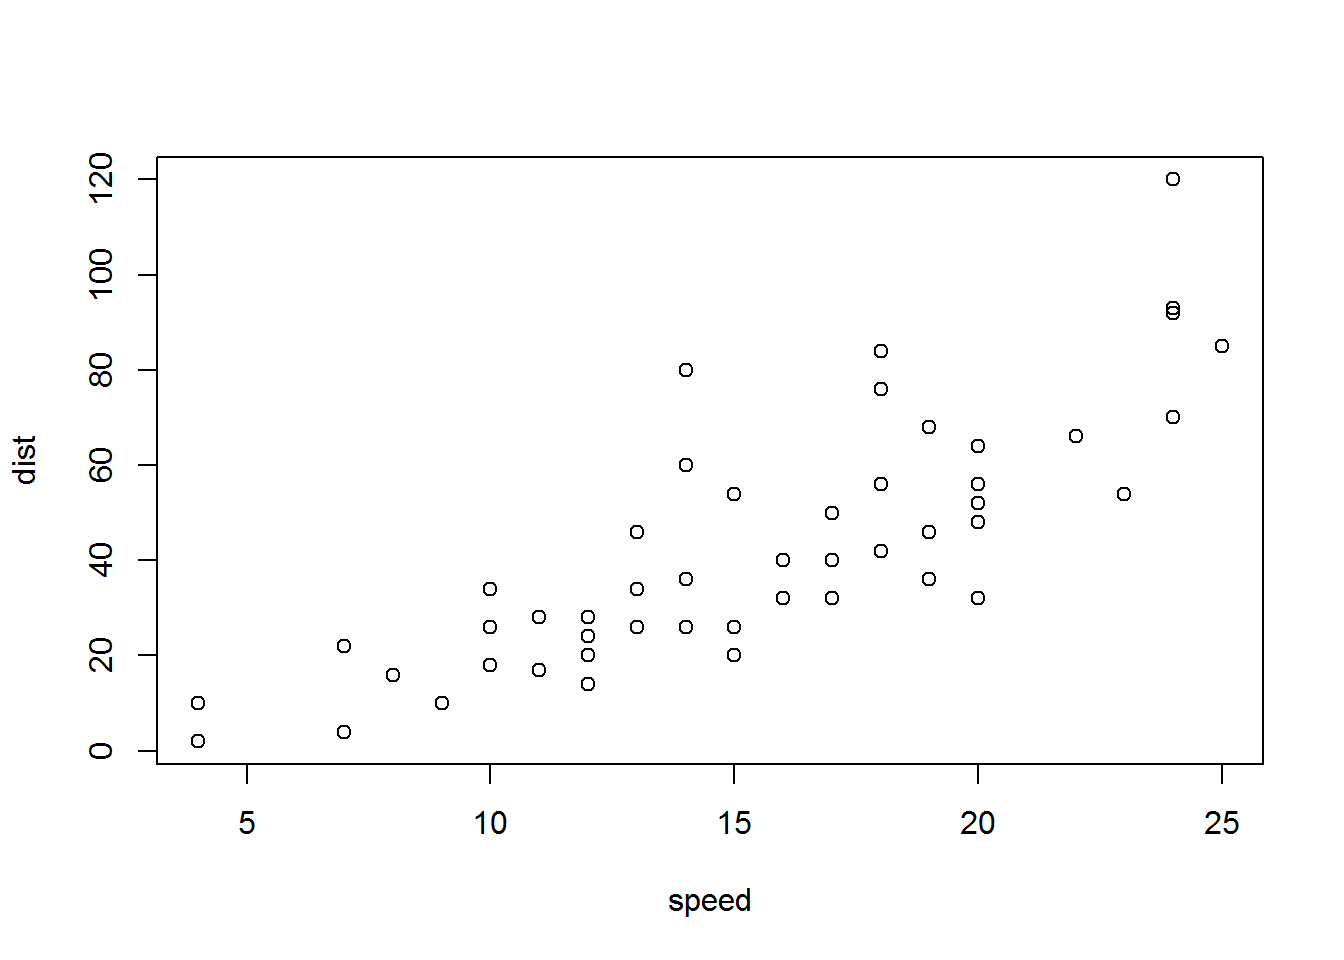
\includegraphics[width=0.8\linewidth]{copernicus2_files/figure-latex/fig1-1} 

}

\caption{caption}\label{fig:fig1}
\end{figure}

Tab. \ref{tab:tab1} psum dolor sit amet, consectetur adipiscing elit,
sed do eiusmod tempor incididunt ut labore et dolore magna aliqua.

\begin{table}

\caption{\label{tab:tab1}Here is a nice table!}
\centering
\begin{tabular}[t]{rrrrl}
\toprule
Sepal.Length & Sepal.Width & Petal.Length & Petal.Width & Species\\
\midrule
5.1 & 3.5 & 1.4 & 0.2 & setosa\\
4.9 & 3.0 & 1.4 & 0.2 & setosa\\
4.7 & 3.2 & 1.3 & 0.2 & setosa\\
4.6 & 3.1 & 1.5 & 0.2 & setosa\\
5.0 & 3.6 & 1.4 & 0.2 & setosa\\
\addlinespace
5.4 & 3.9 & 1.7 & 0.4 & setosa\\
4.6 & 3.4 & 1.4 & 0.3 & setosa\\
5.0 & 3.4 & 1.5 & 0.2 & setosa\\
4.4 & 2.9 & 1.4 & 0.2 & setosa\\
4.9 & 3.1 & 1.5 & 0.1 & setosa\\
\addlinespace
5.4 & 3.7 & 1.5 & 0.2 & setosa\\
4.8 & 3.4 & 1.6 & 0.2 & setosa\\
4.8 & 3.0 & 1.4 & 0.1 & setosa\\
4.3 & 3.0 & 1.1 & 0.1 & setosa\\
5.8 & 4.0 & 1.2 & 0.2 & setosa\\
\addlinespace
5.7 & 4.4 & 1.5 & 0.4 & setosa\\
5.4 & 3.9 & 1.3 & 0.4 & setosa\\
5.1 & 3.5 & 1.4 & 0.3 & setosa\\
5.7 & 3.8 & 1.7 & 0.3 & setosa\\
5.1 & 3.8 & 1.5 & 0.3 & setosa\\
\bottomrule
\end{tabular}
\end{table}

\conclusions

Lorem ipsum dolor sit amet, consectetur adipiscing elit, sed do eiusmod
tempor incididunt ut labore et dolore magna aliqua. Ut enim ad minim
veniam, quis nostrud exercitation ullamco laboris nisi ut aliquip ex ea
commodo consequat. Duis aute irure dolor in reprehenderit in voluptate
velit esse cillum dolore eu fugiat nulla pariatur. Excepteur sint
occaecat cupidatat non proident, sunt in culpa qui officia deserunt
mollit anim id est laborum

\begin{acknowledgements}
Lorem ipsum dolor sit amet, consectetur adipiscing elit, sed do eiusmod
tempor incididunt ut labore et dolore magna aliqua.
\end{acknowledgements}

\bibliography{bib/bib.bib}

\end{document}
